\section{Core Tradeoffs and Representation: RQ1 and RQ2}
\label{sec:empirical_results}

We first report our empirical findings for Research Questions 1 and 2 on the retained 25,228-identifier graph, spanning multi-budget trade-offs, multi-homing mechanics, and representation fidelity.

Figure~\ref{fig:q1_source_partition} partitions covered endpoints by whether any unselected source remains.

\begin{figure}[t]
\centering
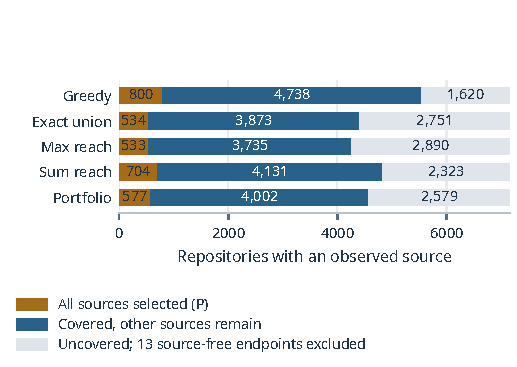
\includegraphics[width=\columnwidth]{coverage_partition.pdf}
\caption{Budget-100 repository partition. Each bar separates all-source exclusion, coverage with residual sources, and uncovered endpoints. The 13 source-free endpoints are omitted. Structural coverage and complete exclusion differ for every baseline.}
\label{fig:q1_source_partition}
\end{figure}

\subsection{RQ1: Coverage vs. Additive Exposure Trade-Off}
Figure~\ref{fig:objective_tradeoff} shows the coverage and exposure trajectories. Table~\ref{tab:multi_budget_comparison} reports empirical prioritization outcomes across maintainer budgets $|S| \in \{1, 5, 10, 25, 50, 100\}$. The top 100 maintainers represent only $0.819\%$ of the 12,217 unique maintainers in our ecosystem, yet their prioritization commands vast reach over downstream workflow repositories.

% Generated by scripts/reconcile_full_manuscript.py
\begin{table*}[t]
\centering
\footnotesize
\caption{Workflow-repository outcomes from the retained baseline experiment. Random entries are 200-order sample means and Monte Carlo standard errors, not population confidence intervals.}
\label{tab:multi_budget_comparison}
\begin{tabular}{llrrrrrr}
\toprule
Budget & Metric & Portfolio & Sum & Max & Exact union & Greedy & Random mean $\pm$ MCSE\\
\midrule
1 & C (\%) & 23.43 & 33.02 & 28.75 & 35.46 & 35.46 & 0.65 $\pm$ 0.19\\
1 & H (\%) & 0.36 & 0.51 & 0.45 & 0.55 & 0.55 & 0.01 $\pm$ 0.00\\
1 & P & 1 & 26 & 2 & 269 & 269 & 0.28 $\pm$ 0.15\\
5 & C (\%) & 46.00 & 49.25 & 42.14 & 50.96 & 54.00 & 2.61 $\pm$ 0.36\\
5 & H (\%) & 1.16 & 2.15 & 2.23 & 2.45 & 2.09 & 0.04 $\pm$ 0.01\\
5 & P & 316 & 325 & 80 & 329 & 327 & 0.69 $\pm$ 0.17\\
10 & C (\%) & 47.90 & 51.75 & 42.81 & 54.53 & 60.40 & 4.73 $\pm$ 0.46\\
10 & H (\%) & 1.59 & 2.68 & 4.06 & 4.48 & 3.79 & 0.08 $\pm$ 0.01\\
10 & P & 391 & 399 & 111 & 343 & 351 & 1.21 $\pm$ 0.19\\
25 & C (\%) & 56.71 & 60.95 & 45.29 & 59.74 & 67.69 & 10.15 $\pm$ 0.55\\
25 & H (\%) & 4.38 & 7.45 & 9.00 & 9.86 & 6.08 & 0.21 $\pm$ 0.01\\
25 & P & 430 & 480 & 116 & 427 & 514 & 2.86 $\pm$ 0.26\\
50 & C (\%) & 62.00 & 63.78 & 45.56 & 60.26 & 72.46 & 16.73 $\pm$ 0.56\\
50 & H (\%) & 6.14 & 13.72 & 17.19 & 18.09 & 8.73 & 0.43 $\pm$ 0.02\\
50 & P & 503 & 576 & 117 & 441 & 638 & 5.97 $\pm$ 0.38\\
100 & C (\%) & 63.85 & 67.42 & 59.52 & 61.46 & 77.23 & 23.44 $\pm$ 0.52\\
100 & H (\%) & 7.96 & 21.98 & 33.59 & 33.79 & 11.48 & 0.80 $\pm$ 0.03\\
100 & P & 577 & 704 & 533 & 534 & 800 & 12.78 $\pm$ 1.42\\
\bottomrule
\end{tabular}
\end{table*}



\begin{figure*}[t]
\centering
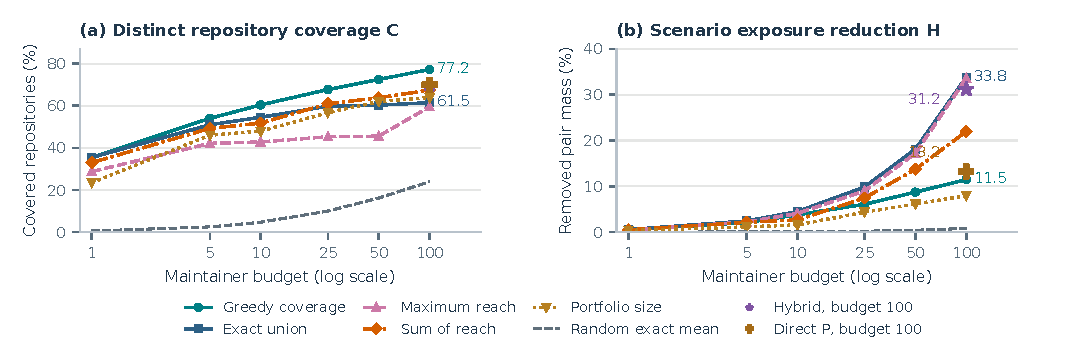
\includegraphics[width=0.92\textwidth]{objective_tradeoff.pdf}
\caption{Multi-budget trade-off trajectories across maintainer budgets $|S| \in [1, 100]$: (a) submodular coverage $C(S)$, (b) modular scenario exposure reduction $H(S)$, using five deterministic rules and the exact random expectation. Budget-100 markers show hybrid and direct-exclusion selections.}
\label{fig:objective_tradeoff}
\end{figure*}

At budget $|S|=100$, \textbf{Greedy Coverage} achieves $C(S) = 5{,}538$ repositories ($77.23\%$), establishing a descriptive lead of $+1{,}131$ repositories ($+15.77$ percentage points) over \textbf{Exact Union} ($C(S) = 4{,}407$, $61.46\%$). However, when evaluated under scenario-weighted additive exposure reduction $H(S)$, Exact Union achieves $33.79\%$, outpacing Greedy Coverage ($11.48\%$) by \textbf{$+22.30$ percentage points} ($2.94\times$ relative advantage).

Exact union's H advantage follows from its additive objective under equal costs. The experiment measures the accompanying loss in distinct coverage. Greedy offers the largest measured coverage among the compared baseline selections; it is an approximation to maximum coverage, not a proved global optimum. Portfolio size gives 63.85\% coverage and 7.96\% H at this budget, showing that portfolio count and measured downstream reach need not agree.

\subsection{Residual Sources and Single-Source Fragility}
A repository can have many source accounts even when a single account already covers it. Across the 7,158 repositories with observed sources, mean source cardinality is 64.57 and the maximum is 1,502. These are graph source identities, not measured permissions or independent compromises. Figure~\ref{fig:q1_source_distribution} shows their distribution and the remaining-source distributions after budget-100 selections.

\begin{figure*}[t]
\centering
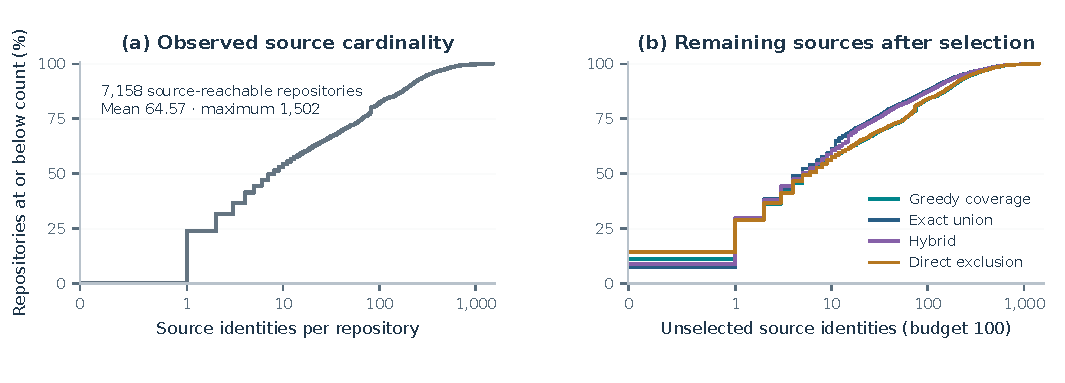
\includegraphics[width=0.94\textwidth]{source_multiplicity.pdf}
\caption{Observed source multiplicity and residual-source distributions at budget 100. All curves use the same 7,158 source-reachable repositories; 13 source-free endpoints are excluded. Zero remaining sources identify all-source exclusions. Horizontal scales are logarithmic above one. Account origins are structural scenarios, not observed compromises.}
\label{fig:q1_source_distribution}
\end{figure*}

Greedy's $P=800$ is 11.18\% of source-reachable repositories; exact union gives $P=534$. Consequently, 6,358 source-reachable repositories retain at least one unselected source after greedy selection. A four-source illustration would retain three source identities when one is selected, but that fraction is not an estimated compromise probability.

\begin{figure}[t]
\centering
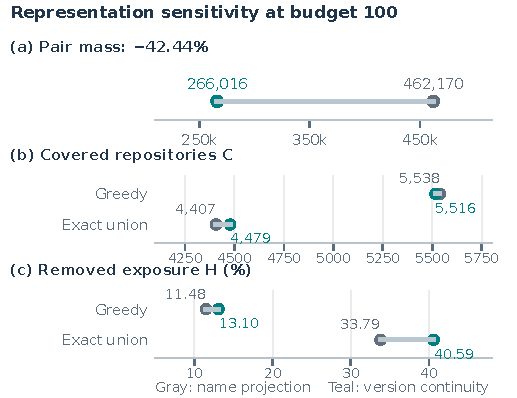
\includegraphics[width=\columnwidth]{representation_detail.pdf}
\caption{Cross-representation divergence: preserving exact-version continuity removes some paths introduced by version merging and reduces total identity-repository exposure pairs by $42.44\%$, shifting maintainer leverage. Gray denotes name projection and teal denotes version continuity.}
\label{fig:representation_detail}
\end{figure}

\subsection{RQ2: Version-Continuity Representation and Selection Penalties}
Figure~\ref{fig:representation_detail} summarizes pair mass and budget-100 outcomes under the two representations.
Comparing the package-projected name graph against the observed exact-version edge union reveals substantial sensitivity to representation:
\begin{enumerate}
    \item \textbf{Exposure Shrinkage:} Preserving version continuity contracts total maintainer-repository exposure pairs from $462{,}170$ to $266{,}016$---an exact reduction of \textbf{$42.44\%$}.
    \item \textbf{Root Scope Changes:} $8{,}587$ out of $25{,}228$ graph identifiers ($34.04\%$) exhibit divergent downstream reach scopes between name-collapsed and version-continuous representations.
    \item \textbf{Cycle Condensation:} Kosaraju condensation detects $403$ nodes in $82$ nontrivial strongly connected components in the name graph, compared to $68$ cyclic components across $40{,}806$ version nodes in the version-continuous graph.
    \item \textbf{Version-Splicing Witnesses:} Retained representation diagnostics include five illustrative roots whose name-level paths lack a continuous counterpart in the retained version graph: \texttt{pseudomap}, \texttt{is}, \texttt{foreach}, \texttt{indexof}, and \texttt{has-color}.
\end{enumerate}

\subsubsection{The Cross-Representation Selection Penalty}
When maintainers are selected based on name-projected heuristics but evaluated on the observed version-continuous graph, measured exposure changes. For the \texttt{sum\_package\_reach} heuristic at budget 100, ranking directly on version-continuous topologies captures \textbf{$34.34\%$} of version exposure, compared to only \textbf{$20.91\%$} when using name-projected rankings---an improvement of \textbf{$+13.43$ percentage points} ($+64.2\%$ relative gain).

\subsubsection{Cross-Sectional Incident-Associated Illustrations}
Table~\ref{tab:q1_incident_case_study} details reach metrics and maintainer prioritization ranks across the 16 incident-associated records whose package names occur in the retained graph.

% Generated by scripts/reconcile_full_manuscript.py
\begin{table*}[t]
\centering
\footnotesize
\caption{Representation sensitivity for 16 retained incident assessments (15 package names). Maintainer ranks now use workflow-repository endpoints throughout.}
\label{tab:q1_incident_case_study}
\begin{tabular}{lllrrrrrrr}
\toprule
Package & Focal maintainer & Ref. version & Dependents & Name reach & Version reach & Portfolio & Greedy & Union & Hybrid\\
\midrule
\texttt{debug} & \texttt{qix} & 4.4.1 & 541/3,525 & 1,462 & 1,162 & \#2,298 & \#>100 & \#7 & \#35\\
\texttt{chalk} & \texttt{sindresorhus} & 5.6.0 & 544/3,416 & 1,125 & 587 & \#2 & \#1 & \#1 & \#1\\
\texttt{ansi-styles} & \texttt{sindresorhus} & 6.2.1 & 25/4,052 & 1,376 & 740 & \#2 & \#1 & \#1 & \#1\\
\texttt{simple-swizzle} & \texttt{qix} & 0.2.2 & 1/357 & 120 & 31 & \#2,298 & \#>100 & \#7 & \#35\\
\texttt{backslash} & \texttt{qix} & 0.2.0 & 1/1 & 0 & 0 & \#2,298 & \#>100 & \#7 & \#35\\
\texttt{eslint-config-prettier} & \texttt{lydell} & 10.1.5 & 14/15 & 10 & 10 & \#561 & \#41 & \#102 & \#31\\
\texttt{eslint-plugin-prettier} & \texttt{lydell} & 5.2.3 & 6/7 & 5 & 5 & \#561 & \#41 & \#102 & \#31\\
\texttt{@solana/web3.js} & \texttt{solana-devs} & 2.1.0* & 6/31 & 4 & 4 & \#181 & \#>100 & \#1,752 & \#465\\
\texttt{nx} & \texttt{jameshenry} & 21.5.0* & 5/52 & 2 & 2 & \#31 & \#>100 & \#835 & \#1,171\\
\texttt{node-ipc (v12)} & \texttt{riaevangelist} & 12.0.0 & 2/4 & 4 & 4 & \#2,562 & \#>100 & \#3,163 & \#1,274\\
\texttt{node-ipc (v10)} & \texttt{riaevangelist} & 10.1.0 & 2/4 & 4 & 4 & \#2,562 & \#>100 & \#3,163 & \#1,274\\
\texttt{@tanstack/history} & \texttt{tannerlinsley} & 1.114.15 & 3/13 & 1 & 1 & \#163 & \#>100 & \#1,423 & \#455\\
\texttt{@ctrl/tinycolor} & \texttt{scttcper} & 4.1.0 & 7/455 & 10 & 9 & \#5,765 & \#>100 & \#2,333 & \#1,227\\
\texttt{@opensearch-project/opensearch} & \texttt{peterzhuamazon} & 3.6.0 & 0/0 & 0 & 0 & \#2,548 & \#>100 & \#1,491 & \#2,323\\
\texttt{@mastra/core} & \texttt{tylerbarnes} & 0.0.0* & 0/0 & 0 & 0 & \#416 & \#>100 & \#6,314 & \#6,697\\
\texttt{echarts-for-react} & \texttt{atool} & 3.0.0 & 0/0 & 0 & 0 & \#398 & \#>100 & \#1,945 & \#747\\
\bottomrule
\end{tabular}
\par\smallskip\begin{minipage}{0.98\textwidth}\footnotesize Reach unions all retained versions; the reference-version label does not restrict the graph. Package reach excludes the root; maintainer reach includes eligible seeds. Focal maintainers are observed members, not necessarily the compromised publisher. A star denotes assessment shorthand. Repeated package assessments are not independent incidents. Rankings and graph fields are not time-aligned forecasts.\end{minipage}
\end{table*}


The individual-package comparison shows representation-dependent reach: \texttt{simple-swizzle} has 120 name-projected and 31 exact-version-continuous workflow endpoints; \texttt{chalk} has 1,125 and 587; \texttt{ansi-styles} has 1,376 and 740; \texttt{debug} has 1,462 and 1,162. These differences do not prove which paths an actual installation could execute.

The account-level example uses the same workflow endpoint definition. \texttt{qix} reaches \QixNameReach{} workflow repositories and ranks \#\QixUnionRank{} by exact union; version continuity yields \QixVersionReach{} and rank \#\QixVersionRank{}. It is beyond greedy's first 100 selections, while the hybrid places it \#\QixHybridRank{}. This illustrates overlap in current retained memberships, not a successful pre-event forecast or historical publisher attribution.

\begin{figure*}[t]
\centering
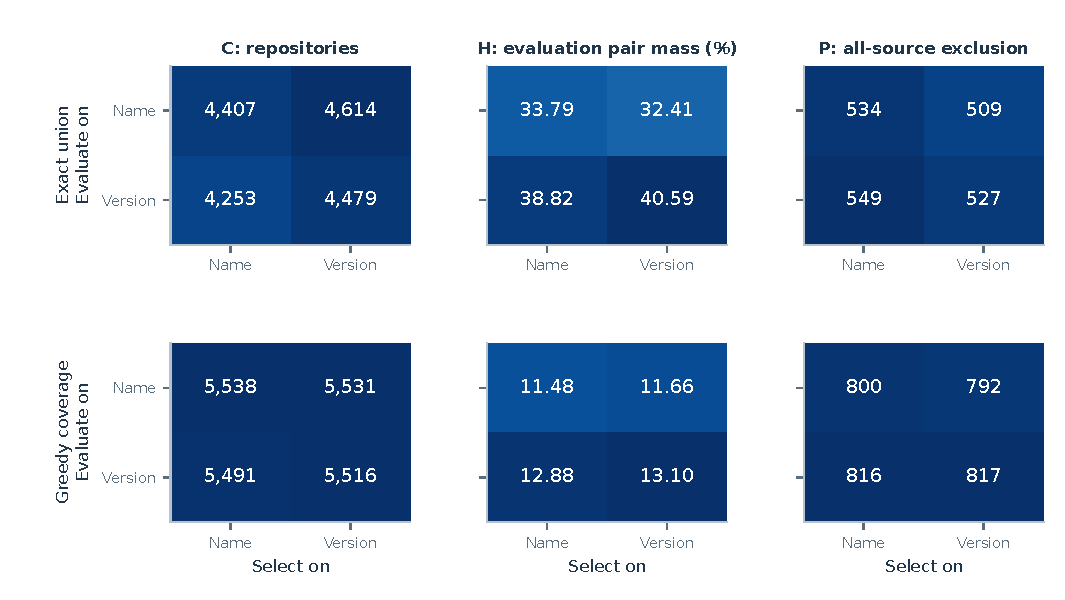
\includegraphics[width=0.98\textwidth]{representation_matrix.pdf}
\caption{Budget-100 selection/evaluation combinations for exact union and greedy. C and P count workflow repositories; H is divided by all account--repository pairs in the evaluation representation (462,170 for names; 266,016 for versions). Panels are separate metrics, not a common color scale.}
\label{fig:q1_representation_matrix}
\end{figure*}

Figure~\ref{fig:q1_representation_matrix} separates the representation used for selection from the one used for evaluation. Comparisons of H within an evaluation row share a denominator; comparisons across rows change that denominator. A change in representation can therefore change both the selection and the quantity being measured.
